\section{Sprint Goal}

Figure \ref{fig:design} shows the software design we choose for our
project, and how the system interacts with the user. The yellow boxes
are the given sites and the green boxes is the databases of the sites.
The red User box represents the User actor. As of the start of the project
the Leapkit Frontend, Leapkit Projects, Leapkit Users are already implemented by 
our product owner.
This means the yellow and red boxes also represents our general architecture.

\begin{figure}[h]
    \centering
    \usetikzlibrary{shadows,arrows}
% Define the layers to draw the diagram
\pgfdeclarelayer{background}
\pgfdeclarelayer{foreground}
\pgfsetlayers{background,main,foreground}
 
% Define block styles  
\tikzstyle{rectangle}=[draw, fill=blue!20, text width=6.0em, text centered,
  minimum height=1.5em,drop shadow]
\tikzstyle{practica} = [rectangle, text width=8em, minimum width=10em,
  minimum height=3em, rounded corners, drop shadow]

\tikzstyle{circle}=[draw, fill=green!20, text width=6.0em, text centered,
  minimum height=1.5em,drop shadow]
\tikzstyle{interface} = [circle, text width=8em, minimum width=10em,
  minimum height=3em, rounded corners, drop shadow]
 
\tikzstyle{texto} = [above, text width=6em, text centered]
\tikzstyle{linepart} = [draw, thick, color=black!50, -latex', dashed]
\tikzstyle{line} = [draw, thick, color=black!50, -latex']
\tikzstyle{ur}=[draw, text centered, minimum height=0.01em]
 
% Define distances for bordering
\newcommand{\blockdist}{1.3}
\newcommand{\edgedist}{1.5}

\newcommand{\practica}[3]{node (p#1) [practica] {#2 \\ \scriptsize\textit{#3}}}
\newcommand{\implemented}[3]{node (p#1) [interface] {#2 \\ \scriptsize\textit{#3}}}

% Draw background
\newcommand{\background}[5]{%
  \begin{pgfonlayer}{background}
    % Left-top corner of the background rectangle
    \path (#1.west |- #2.north)+(-0.5,0.5) node (a1) {};
    % Right-bottom corner of the background rectanle
    \path (#3.east |- #4.south)+(+0.5,-0.25) node (a2) {};
    % Draw the background
    \path[fill=yellow!20,rounded corners, draw=black!50, dashed]
      (a1) rectangle (a2);
    \path (a1.east |- a1.south)+(0.8,-0.3) node (u1)[texto]
      {\scriptsize\textit{#5}};
  \end{pgfonlayer}}

\newcommand{\transreceptor}[3]{%
  \path [linepart] (#1.east) -- node [above]
    {\scriptsize Transreceptor #2} (#3);}

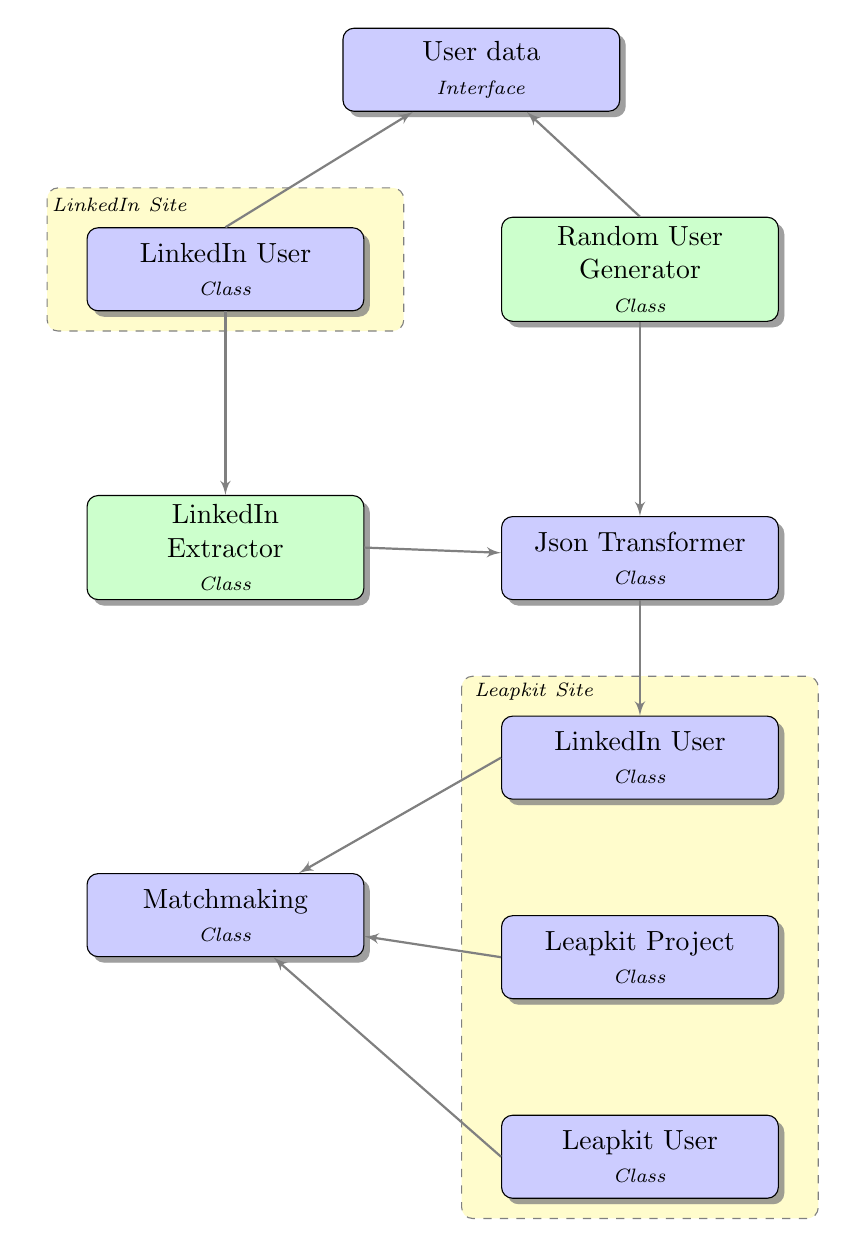
\begin{tikzpicture}


% Draw diagram elements
\path                        \practica{1}{User data}{Interface};
\path (p1.south)+(-3.25,-2.0) \practica{2}{LinkedIn User}{Class};
\path (p2.east) +( 3.5, 0.0) \implemented{3}{Random User Generator}{Class};

\path (p2.south) +( 0.0,-3.0) \implemented{4}{LinkedIn Extractor}{Class};
\path (p3.south) +( 0.0,-3.0) \practica{5}{Json Transformer}{Class};


\path (p5.south)+(0.0,-2.0) \practica{6}{LinkedIn User}{Class};
\path (p6.south)+(0.0,-2.0) \practica{7}{Leapkit Project}{Class};
\path (p7.south)+(0.0,-2.0) \practica{8}{Leapkit User}{Class};
 
\path (p4.south)+(0.0,-4.0) \practica{9}{Matchmaking}{Class};
% \path (p6.south)+(2.5,-1.25) \practica{8}{Demodulador AM};
% \path (p8.east)+(+5.5,0) node (ur1)[ur] {};

% \path (p7.south)+(0.0,-1.5) \practica{9}{Codificador digital};
% \path (p8.south)+(0.0,-1.5) \practica{10}{Decodificador digital};
% \path (p10.east)+(+5.5,0) node (ur2)[ur] {};
% \path (p9.south)+(0.0,-1.5) \practica{11}{Codificador FDM};
% \path (p10.south)+(0.0,-1.5) \practica{12}{Decodificador FDM};
% \path (p12.east)+(+5.5,0) node (ur3)[ur] {};
% \path (p11.south)+(0.0,-1.5) \practica{13}{Codificador SSTV};
% \path (p12.south)+(0.0,-1.5) \practica{14}{Decodificador SSTV};
% \path (p14.east)+(+5.5,0) node (ur4)[ur] {};
% \path (p14.south)+(-2.5,-1.5) \practica{15}{Conmutaci\'on telef\'onica};
% \path (p15.south)+(0.0,-1.0) \practica{16}{Telfon\'ia celular an\'aloga};
% \path (p16.south)+(0.0,-1.5) \practica{17}{Receptor de  telemetr\'ia}; 
% \path (p17.south)+(0.0,-1.5) \practica{18}{Gu\'ias de ondas};

% Draw arrows between elements
\path [line] (p2.north) -- node [above] {} (p1);
\path [line] (p3.north) -- node [above] {} (p1);

\path [line] (p2.south) -- node [above] {} (p4);
\path [line] (p3.south) -- node [above] {} (p5);

\path [line] (p4.east) -- node [above] {} (p5);

\path [line] (p5.south) -- node [above] {} (p6);
\path [line] (p6.west) -- node [above] {} (p9);
\path [line] (p7.west) -- node [above] {} (p9);
\path [line] (p8.west) -- node [above] {} (p9);
% \path [line] (p2.south) -- +(0.0,-0.5) -- +(-2.5,-0.5)
    % -- node [above, midway] {} (p3);
% \path [line] (p3.south) -- node [above] {} (p5) ;

% \path [line] (p2.south) -- +(0.0,-0.5) -- +(+2.5,-0.5)
    % -- node [above, midway] {} (p4);
% \path [linepart] (p3.east) -- +(+0.5,-0.0) -- +(+0.5,-1.75)
    % -- node [left, midway] {} (p4);
% \path [linepart] (p3.east) -- +(+0.5,-0.0) -- +(+0.5,-1.75)
    % -- node [left, midway] {} (p4);

% \path [line] (p4.south) -- +(0.0,-0.5) -- +(-2.5,-0.5)
    % -- node [above, midway] {} (p6);
% \path [line] (p5.south) -- +(0.0,-0.5) -- +(+2.5,-0.5)
    % -- node [above, midway] {} (p6);     
% \path [linepart] (p2.east) -- +(2.75,0.0) -- +(2.75,-5.85)
    % -- node [right] {} (p6);
% \path [line] (p6.south) -- +(0.0,-0.25) -- +(-2.5,-0.25)
    % -- node [above, midway] {} (p7);
% \path [line] (p6.south) -- +(0.0,-0.25) -- +(+2.5,-0.25)
    % -- node [above, midway] {} (p8);
% \path [linepart] (p7.east) -- node [left] {} (p8);
% \transreceptor{p8}{AM banda 40m}{ur1}

% \path [line] (p7.south) -- node [above] {} (p9) ;
% \path [line] (p8.south) -- node [above] {} (p10) ;
% \path [linepart] (p9.east) -- node [left] {} (p10);
% \transreceptor{p10}{CW}{ur2}
% \path [line] (p9.south) -- node [above] {} (p11) ;
% \path [line] (p10.south) -- node [above] {} (p12) ;
% \path [linepart] (p11.east) -- node [left] {} (p12);
% \transreceptor{p12}{FDMDV}{ur3}

% \path [line] (p11.south) -- node [above] {} (p13) ;
% \path [line] (p12.south) -- node [above] {} (p14) ;
% \path [linepart] (p13.east) -- node [left] {} (p14);   
% \transreceptor{p14}{SSTV}{ur4}

% \path [line] (p14.south) -- +(0.0,-0.5) -- +(-2.5,-0.5)
    % -- node [above, midway] {} (p15);
% \path [line] (p13.south) -- +(0.0,-0.5) -- +(+2.5,-0.5)
    % -- node [above, midway] {} (p15);
% \path [line] (p15.south) -- node [above] {} (p16) ;     
% \path [line] (p16.south) -- node [above] {} (p17) ;
% \path [line] (p17.south) -- node [above] {} (p18) ;

\background{p2}{p2}{p2}{p2}{LinkedIn Site}
\background{p6}{p6}{p8}{p8}{Leapkit Site}

% \background{p3}{p3}{p4}{p5}{II}
% \background{p3}{p6}{p4}{p7}{III}
% \background{p3}{p9}{p4}{p10}{IV}
% \background{p3}{p11}{p4}{p12}{V}
% \background{p3}{p13}{p4}{p14}{VI}
% \background{p3}{p15}{p4}{p16}{VII}
% \background{p3}{p17}{p4}{p17}{VIII}
% \background{p3}{p18}{p4}{p18}{IX}
\end{tikzpicture}

    \caption{Software design}
    \label{fig:design}
\end{figure}
